\section{Experiments}
\label{sec:exp}
\vspace{-0.5em}
This paper introduces a novel concept called temporally coupled attacks, which distinguishes itself from standard adversarial attacks by incorporating temporal coupling. Previous research has primarily focused on attackers with different functionalities, specifically targeting either the state space or the action space. In our experimental setup, we investigate three types of attackers: those specialized in perturbing the state space, those focused on perturbing the action space, and those capable of adaptably targeting both spaces. Within each attack domain, we consider both the standard attackers without temporal coupling and the temporally-coupled attackers. By employing this diverse set of attackers, we conduct a comprehensive evaluation of the state-of-the-art robustness of our proposed method, \ours, in comparison to existing robust baselines. This evaluation sheds light on the effectiveness of \ours across a wide range of attack scenarios and highlights its robustness against different types of adversaries.

\textbf{Experiment setup.} 
Our experiments are conducted on five various and challenging MuJoCo environments: Hopper, Walker2d, Halfcheetah, Ant, and Humanoid, all using the v2 version of MuJoCo. We use the Proximal Policy Optimization (PPO) algorithm as the policy optimizer and a Long Short-Term Memory (LSTM) network as the policy network for all of the robust training methods we evaluate. To maintain methodological consistency and minimize potential discrepancies arising from different PPO implementations across methods, we ensure highly similar benchmark results. For attack constraint $\epsilon$, we use the commonly adopted values $\epsilon$ for each environment. For the temporally-coupled constraint $\bar{\epsilon}$, we set the optimal maximum $\bar{\epsilon}$ as $\epsilon/5$ (with minor adjustments in some environments). Other choices of $\bar{\epsilon}$ will be further discussed in the ablation studies.

In terms of evaluation metrics, we report the average test episodic rewards both under no attack and against the strongest adversarial attacks to reflect both the natural performance and robustness of trained agents, by training adversaries targeting the trained agents from scratch. For reproducibility, we train each agent configuration with 10 seeds and report the one with the median robust performance, rather than the best one. More implementation details are in Appendix~\ref{app:exp:imp}.

\textbf{Baselines.} 
We compare our approach \ours with other robust RL baselines in this paper. Robust training frameworks can be categorized into two types. The first type requires training with a specified adversary during training, such as the alternating training framework (ATLA~\citep{zhang2021robust}) and \ours. The second type does not require training with an adversary, such as WocaR-PPO~\citep{liang2022efficient} and AR-PPO (PPO variant of AR-DDPG~\citep{tessler2019action}). The baselines we chose demonstrate state-of-the-art or great robustness in prior works. The first type of approaches require training agents with adversaries targeting specific attack domains and the second type of baselines can be evaluated directly for their robustness without the need for additional adversary training.

\textbf{Case I: Against attacks on state space}

In this experiment, our focus is on evaluating the robustness of our methods against state adversaries that perturb the states received by the agent. Among the ATLA~\citep{zhang2021robust, sun2021strongest} methods, PA-ATLA-PPO is the most robust, which trains with the standard strongest PA-AD attacker. As a modification, we train PA-ATLA-PPO* with a temporally-coupled PA-AD attacker. For a more intuitive and fair comparison, in Table~\ref{tab:table_state} we only present the rewards of the best-performing ATLA agents under the type of attacks they were trained with. Our \ours method utilizes the temporally-coupled PA-AD attacker for training. We report the lowest rewards achieved under both standard and temporally-coupled state attacks among the six existing strongest adversaries to present the robustness of robust models.

In the absence of any attacks, \ours maintains a competitive natural reward, which indicates that the agent's performance does not degrade significantly in the environment where is no adversary after approaching an approximate Nash equilibrium with the adversary. Even without training with regular attackers, our method demonstrates significantly better robustness under the non-temporally-coupled type of attack, particularly in the highest-dimensional and challenging environment, Humanoid, where it outperforms other methods by a large margin. Under our proposed temporally-coupled attacks, the average performance of our approach surpasses the state-of-the-art by up to 45\%, highlighting the strong robustness of the policies learned by \ours against all types of state adversarial attacks.
% \begingroup
% \setlength{\tabcolsep}{6pt} % Default value: 6pt
% \renewcommand{\arraystretch}{1} 
% \begin{table*}[ht!]
% \centering
%   \caption{State of the \texttt{AC} first version VS State of the \texttt{AC} second version}
% \label{tbl:toyExampleStates}
% \resizebox{\linewidth}{!} {
% \begin{tabular}{l|l|l|c|c|c|c|c|c|c|c|c|c|c|c}
% \toprule
% \multirow{2}{*}{\textbf{test$_{ID}$}}& 
% \multirow{2}{*}{\textbf{Input}}& 
% \multirow{2}{*}{\textbf{MC$^\star$}} & 
% \multicolumn{6}{c|}{\textbf{\texttt{AC} version 1}} & 
% \multicolumn{6}{c}{\textbf{\texttt{AC} version 2}}  \\
%  &  &  & get\_last & get\_first & get\_size & is\_empty & sum & average & get\_last & get\_first & get\_size & is\_empty & sum & average \\
% \midrule
% \multirow{5}{*}{test\_sum}  &	[2, 3, 1, 4, 5]	&	sum	    &	5	&	2	& 5	&	FALSE	&	15	&	3	&	5	&	2	&	5	&	FALSE	&	15	&	3	\\
%                       	&	[5, 4, 1, 3, 2]	&	reverse	&	2	&	\textbf{5}	& 5	&	FALSE	&	15	&	3	&	3	&	\textbf{2}	&	5	&	FALSE	&	15	&	3	\\
%                 &	[5, 4, 1, 3, 2, 6, 7, 8]	&	append	&	8	&	\textbf{5}	& 8	&	FALSE	&	36	&	4.5	&	8	&	\textbf{2}	&	8	&	FALSE	&	36	&	4.5	\\
%             &	[5, 4, 1, 3, 2, 6, 7, 8, 9, 10]	&	append	&	10	&	\textbf{5}	& 10&	FALSE	&	55	&	5.5	&	10	&	\textbf{2}	&	10	&	FALSE	&	55	&	5.5	\\
%             &	[5, 4, 1, 3, 2, 6, 7, 8, 9, 10]	&	get	    &	10	&	\textbf{5}	& 10&	FALSE	&	55	&	5.5	&	10	&	\textbf{2}	&	10	&	FALSE	&	55	&	5.5	\\
% \midrule

% \multirow{6}{*}{test\_avg}  & [2, 3, 1, 4, 5]	&	CTOR	&	-	&	-	-	&	-	&	-	&	-	&	-	&	-	&	-	&	-	&	-	&	-	\\
% & [2, 3, 1, 4, 5]	        &	average	&	5	&	2	& 5	&	FALSE	&	15	&	3	&	5	&	2	&	5	&	FALSE	&	15	&	3	\\
% & [5, 4, 1, 3, 2]	        &	reverse	&	\textbf{2}	&	\textbf{5}	& 5	&	FALSE	&	15	&	3	&	\textbf{3}	&	\textbf{2}	&	5	&	FALSE	&	15	&	3	\\
% & [5, 4, 1, 3, 2, 6, 7, 8]	&	append	&	8   &	\textbf{5}	& 8	&	FALSE	&	36	&	4.5	&	8	&	\textbf{2}	&	8	&	FALSE	&	36	&	4.5	\\
% & [8, 7, 6, 2, 3, 1, 4, 5]	&	reverse	&	5	&	\textbf{8}   & 8	&	FALSE	&	36	&	4.5	&	5	&	\textbf{2}	&	8	&	FALSE	&	36	&	4.5	\\
% & [8, 7, 6, 2, 3, 1, 4, 5]	&	average	&	5	&	\textbf{8}   & 8	&	FALSE	&	36	&	4.5	&	5	&	\textbf{2}	&	8	&	FALSE	&	36	&	4.5	\\

% \midrule
% \multirow{2}{*}{{test\_average\_empty }} & [2, 3, 1, 4, 5]	&	CTOR	&	-	&	- &	-	&	-	&	-	&	-	&	-	&	-	&	-	&	-	&	-	&	-	\\
%                                           & []	&	clear	&		&	&	0	&	TRUE	&	0	&		&		&		&	0	&	TRUE	&	0	&		\\
% \bottomrule
% \multicolumn{5}{l}{$^\star$Method call during test execution}
% \end{tabular}}
% \end{table*}%
% \endgroup

\begingroup
\setlength{\tabcolsep}{6pt} % Default value: 6pt
\renewcommand{\arraystretch}{1} 
\begin{table*}[ht!]
\centering
  \caption{State data of the \texttt{AC} class first version VS State data of the \texttt{AC} class second version}
\label{tbl:toyExampleStates}
\resizebox{\linewidth}{!} {
\begin{tabular}{l|l|l|c|c|c|c|c|c|c|c|c|c|c|c}
\toprule
\multirow{2}{*}{\textbf{test$_{ID}$}}& 
\multirow{2}{*}{\textbf{Input}}& 
\multirow{2}{*}{\textbf{MC$^\star$}} & 
\multicolumn{6}{c|}{\textbf{\texttt{AC} version 1}} & 
\multicolumn{6}{c}{\textbf{\texttt{AC} version 2 (refactored and buggy)}}  \\
 &  &  & get\_last & get\_first & get\_size & is\_empty & sum & average & get\_last & get\_first & get\_size & is\_empty & sum & average \\
\midrule
\multirow{2}{*}{test\_sum} & \multirow{2}{*}{[2, 3, 1, 4, 5]}	&	
CTOR	&	-	&	-	& -	&	-	&	-	&	-	&	-	&	-	&	-	&	-	&	-	&	-	\\
& 	&	
sum	    &	5	&	2	& 5	&	FALSE	&	15	&	3	&	5	&	2	&	5	&	FALSE	&	15	&	3	\\
\midrule
\multirow{2}{*}{test\_avg}  & \multirow{2}{*}{[2, 3, 1, 4, 5]}	&	CTOR	&	-	&	-	& -	&	-	&	-	&	-	&	-	&	-	&	-	&	-	&	-	&	-	\\
& &	average	&	5	&	2	& 5	&	FALSE	&	15	&	3	&	5	&	2	&	5	&	FALSE	&	15	&	3	\\
\midrule
\multirow{5}{*}{sequence\_one} & \multirow{5}{*}{[2, 3, 1, 4, 5]}	&	CTOR	&	-	&	-	& -	&	-	&	-	&	-	&	-	&	-	&	-	&	-	&	-	&	-	\\	
& &	append	& \textbf{8}	&	2	& 8	&	FALSE	&	36	&	4.5	&	\textbf{7}	&	2	&	8	&	FALSE	&	36	&	4.5	\\
& &	reverse	&	\textbf{2}	&	\textbf{5}	& 5	&	FALSE	&	15	&	3	&	\textbf{4}	&	\textbf{2}	&	5	&	FALSE	&	15	&	3	\\
& &	append	&	\textbf{10}	&	\textbf{5}	& 10&	FALSE	&	55	&	5.5	&	\textbf{9}	&	\textbf{2}	&	10	&	FALSE	&	55	&	5.5	\\
& &	sum	&	\textbf{10}	&	\textbf{5}	& 10&	FALSE	&	55	&	5.5	&	\textbf{9}	&	\textbf{2}	&	10	&	FALSE	&	55	&	5.5	\\

\midrule

\multirow{5}{*}{sequence\_two} & \multirow{5}{*}{[2, 3, 1, 4, 5]} &	CTOR	&	-	&	-	& -	&	-	&	-	&	-	&	-	&	-	&	-	&	-	&	-	&	-	\\
& &	reverse	&	\textbf{2}	&	\textbf{5}	& 5	&	FALSE	&	15	&	3	&	\textbf{4}	&	\textbf{2}	&	5	&	FALSE	&	15	&	3	\\
& &	avg	&	\textbf{2}	&	\textbf{5}	& 5	&	FALSE	&	15	&	3	&	\textbf{4}	&	\textbf{2}	&	5	&	FALSE	&	15	&	3	\\
& &	append	&	\textbf{8}   &	\textbf{5}	& 8	&	FALSE	&	36	&	4.5	&	\textbf{7}	&	\textbf{2}	&	8	&	FALSE	&	36	&	4.5	\\
& &	reverse	&	\textbf{5}	&	\textbf{8}   & 8	&	FALSE	&	36	&	4.5	&	\textbf{7}	&	\textbf{2}	&	8	&	FALSE	&	36	&	4.5	\\

% \midrule
% \multirow{2}{*}{{test\_average\_empty }} & [2, 3, 1, 4, 5]	&	CTOR	&	-	&	- &	-	&	-	&	-	&	-	&	-	&	-	&	-	&	-	&	-	&	-	\\
%                                           & []	&	clear	&		&	&	0	&	TRUE	&	0	&		&		&		&	0	&	TRUE	&	0	&		\\
\bottomrule
\multicolumn{5}{l}{$^\star$Method call during test execution}
\end{tabular}}
\end{table*}%
\endgroup

\textbf{Case II: Against attacks on action space}

In addition to state attacks, we assess the robustness of our methods against action adversaries that perturb the actions taken by the agent. Action perturbations have been extensively studied in the context of model uncertainty in control. In this attack domain, we are the first to train an RL-based action adversary using the trajectory outlined in Algorithm~\ref{alg:ours}, aiming to showcase the worst-case performance of our robust agents under action perturbations.

Among our baselines, we include AR-PPO, although it is not robust against strong action adversaries and performs well only under random noise. Another modification we made is AC-ATLA-PPO, where we train the agent alternately with the aforementioned action adversary. Similar to PA-ATLA-PPO*, we also train AC-ATLA-PPO* agents with a temporally-coupled action adversary, which is also utilized to train our \ours agents. Since RL-based action adversaries lead to a more significant drop in rewards compared to action noise, we report the best action attack rewards achieved by the robust agents under the strongest trained action attacks for robustness evaluation.

In general, while action perturbation may not cause as strong of a "damage" as state perturbation, our \ours method still achieves superior robustness. In terms of natural reward, \ours performs comparably with other baselines. While the advantage of \ours may not be apparent or significant under standard action attacks in less challenging environments, it surpasses other methods by more than 10\% on Ant and Humanoid. Under temporally-coupled action attacks, \ours consistently outperforms the most robust baseline by an average of over 20\%, particularly exhibiting exceptional robustness on Humanoid. These results demonstrate the effective defense of \ours against different types of adversarial attacks in the action space.
\begin{table*}[!t]
\vspace{-0.5em}
\centering
\renewcommand{\arraystretch}{1.2}
\resizebox{\textwidth}{!}{%
\setlength{\tabcolsep}{4pt}
% \setlength{\arrayrulewidth}{1pt}
\begin{tabular}{p{2.5cm}<{\centering} | p{2.7cm}<{\centering}| p{2.5cm}<{\centering}| p{2.5cm}<{\centering}|p{2.5cm}<{\centering}| p{2.5cm}<{\centering}|p{2.5cm}<{\centering}}
\toprule
\multicolumn{2}{c|}{\textbf{Environment}}     & \textbf{Hopper}         & \textbf{Walker2d}  & \textbf{Halfcheetah} & \textbf{Ant} & \textbf{Humanoid} \\
\midrule
\multicolumn{2}{c|}{$\epsilon$ / action dim}     & 0.2 / 3      & 0.2 / 6 & 0.2 / 6 & 0.15 / 8 & 0.15 / 17 \\
\midrule
\multirow{4}{5em}{\begin{tabular}[c]{@{}c@{}}{\textbf{Natural}}\\\textbf{Reward}\\\textbf{(no attack)}\end{tabular}} & AC-ATLA-PPO & 3576 $\pm$ 43  & 4228 $\pm$ 26  & 5915 $\pm$ 28  & 5557 $\pm$ 33 & 6014 $\pm$ 49 \\
&  AC-ATLA-PPO* & 3492 $\pm$ 28 & 4052 $\pm$ 29 & 5853 $\pm$ 32 & 5549 $\pm$ 21 & 5980 $\pm$ 30 \\
&  AR-PPO & 3188 $\pm$ 28 & 3767 $\pm$ 15 &  5248 $\pm$ 35  & 5074 $\pm$ 34  & 5379 $\pm$ 42  \\
&  \textbf{\ours (Ours)} & 3482 $\pm$ 20 & 4159 $\pm$ 26 & 6047 $\pm$ 29 & 5512 $\pm$ 38 & 5894 $\pm$ 35 \\
\midrule
\multirow{4}{5em}{\begin{tabular}[c]{@{}c@{}}{\textbf{Best}}\\\textbf{Standard}\\\textbf{Action Attack}\end{tabular}} 
& AC-ATLA-PPO &  2872  $\pm$ 18  & 3108 $\pm$ 22  & 3994 $\pm$ 41 & 2752 $\pm$ 33 & 3120 $\pm$ 39 \\
&  AR-PPO &  1235 $\pm$ 26 & 1305 $\pm$ 31 & 1523 $\pm$ 24  & 1120 $\pm$ 10  & 1117 $\pm$ 37  \\
&  WocaR-PPO & 2943 $\pm$ 18 & 3269 $\pm$ 28 & 3840 $\pm$ 29 & 3345 $\pm$ 21 & 3419 $\pm$ 37 \\
&  \cellcolor{lightgray}{\textbf{\ours (Ours)}} & \cellcolor{lightgray}{\textbf{3039 $\pm$ 20}} & \cellcolor{lightgray}{\textbf{3298 $\pm$ 35} }& \cellcolor{lightgray}{\textbf{4016 $\pm$ 28}} & \cellcolor{lightgray}{\textbf{3569 $\pm$ 26}} & \cellcolor{lightgray}{\textbf{4106 $\pm$ 32}} \\
\midrule
\multirow{3}{5em}{\begin{tabular}[c]{@{}c@{}}{\textbf{Best}}\\\textbf{Temporally-}\\\textbf{Coupled}\\\textbf{Action Attack}\end{tabular}} & AC-ATLA-PPO* & 2625 $\pm$ 15 & 2780 $\pm$ 26 & 3815 $\pm$ 36 & 3382 $\pm$ 27 & 3092 $\pm$ 17 \\
&  AR-PPO &  974 $\pm$ 15 & 1120 $\pm$ 28 & 1439 $\pm$ 21  & 679 $\pm$ 18  & 585 $\pm$ 29   \\
&  WocaR-PPO & 2673 $\pm$ 28 & 2860 $\pm$ 32 & 4018 $\pm$ 37 & 3260 $\pm$ 27 & 3132 $\pm$ 35 \\
&  \cellcolor{lightgray}{\textbf{\ours (Ours)}} & \cellcolor{lightgray}{\textbf{3125 $\pm$ 26}} & \cellcolor{lightgray}{\textbf{3179 $\pm$ 20} }& \cellcolor{lightgray}{\textbf{4320 $\pm$ 27}} & \cellcolor{lightgray}{\textbf{3619 $\pm$ 34}} & \cellcolor{lightgray}{\textbf{4156 $\pm$ 29}} \\
\bottomrule
\end{tabular}}
% \vspace{-1em}
\caption{Average episode rewards $\pm$ standard error for over 100 episodes action robust baselines and our \textbf{\ours} under no attack and best action attacks. }
\label{tab:table_action}
\vspace{-1.5em}
\end{table*}

\textbf{Case III: Against attacks on either state or action spaces}

In prior works, adversarial attacks typically focus on perturbing either the agent's observations or introducing noise to the action space. However, in real-world scenarios, agents may encounter both types of attacks. To address this challenge, we propose an adversary called the State or Action Adversary (SA-AD), which allows the adversary to choose between attacking the agent's state or action at each time step, integrating this choice into the adversary's action space. The SA-AD attacker, inspired by the PA-AD attacker~\cite{sun2021strongest}, only needs to learn the best policy perturbation directions that can be transformed into state or action perturbations according to the adversary's choices while maintaining manageable training complexity. For further details on the SA-AD attacker, please refer to Appendix~\ref{app:exp:alg}. Similar to the previous experiments, We train SA-ATLA-PPO with SA regular attacker, while SA-ATLA-PPO* and \ours are trained with temporally-coupled SA attackers.

Our experimental results demonstrate that \ours obtains similar natural rewards compared to the ATLA baselines, which is consistent with the findings from previous experiments. To summarize the results under SA attacks, our findings indicate that the combination of two different forms of attacks can effectively target robust agents in most scenarios, providing strong evidence of their robustness. In the case of regular SA attackers, \ours outperforms other methods in all five environments, with a margin of over 20\% in the Humanoid environment. Moreover, when defending against temporally-coupled attacks, \ours significantly enhances robustness by more than 30\% in multiple environments, with a minimum improvement of 10\%. These results clearly demonstrate the robustness of \ours against attackers that can target different domains.
\begin{table*}[!t]
\vspace{-0.5em}
\centering
\renewcommand{\arraystretch}{1.3}
\resizebox{\textwidth}{!}{%
\setlength{\tabcolsep}{4pt}
% \setlength{\arrayrulewidth}{1pt}
\begin{tabular}{p{2.5cm}<{\centering} | p{2.7cm}<{\centering}| p{2.5cm}<{\centering}| p{2.5cm}<{\centering}|p{2.5cm}<{\centering}| p{2.5cm}<{\centering}|p{2.5cm}<{\centering}}
\toprule
\multicolumn{2}{c|}{\textbf{Environment}}     & \textbf{Hopper}         & \textbf{Walker2d}  & \textbf{Halfcheetah} & \textbf{Ant} & \textbf{Humanoid} \\
\midrule
\multirow{3}{5em}{\begin{tabular}[c]{@{}c@{}}{\textbf{Natural}}\\\textbf{Reward}\\\textbf{(no attack)}\end{tabular}} & SA-ATLA-PPO & 3498 $\pm$ 34  & 4195 $\pm$ 36  &  6078 $\pm$ 38  & 5442 $\pm$ 28 & 5913 $\pm$ 34 \\
&  SA-ATLA-PPO* & 3372 $\pm$ 29 & 4219 $\pm$ 31 & 5979 $\pm$ 37 & 5510 $\pm$ 29 & 5949 $\pm$ 22\\
&  \textbf{\ours (Ours)} & 3420 $\pm$ 18 & 4218 $\pm$ 27 & 6123 $\pm$ 18 & 5517 $\pm$ 21 & 5799 $\pm$ 27 \\
\midrule
\multirow{3}{5em}{\begin{tabular}[c]{@{}c@{}}{\textbf{Best}}\\\textbf{Standard}\\\textbf{SA Attack}\end{tabular}} 
& SA-ATLA-PPO & 2294 $\pm$ 27 & 2503 $\pm$ 34 & 4028 $\pm$ 28 & 2750 $\pm$ 32 & 1981 $\pm$ 25 \\
&  WocaR-PPO & 2469 $\pm$ 18 &  2594 $\pm$ 32 &  4012 $\pm$ 26 & 3024 $\pm$ 23  & 2263 $\pm$ 28  \\
&  \cellcolor{lightgray}{\textbf{\ours (Ours)}} & \cellcolor{lightgray}{\textbf{2846 $\pm$ 24}} & \cellcolor{lightgray}{\textbf{2897 $\pm$ 31} }& \cellcolor{lightgray}{\textbf{4168 $\pm$ 37}} & \cellcolor{lightgray}{\textbf{3286 $\pm$ 20}} & \cellcolor{lightgray}{\textbf{3042 $\pm$ 24}} \\
\midrule
\multirow{3}{5em}{\begin{tabular}[c]{@{}c@{}}{\textbf{Best}}\\\textbf{\scriptsize{Temporally-coupled}}\\\textbf{SA Attack}\end{tabular}} & SA-ATLA-PPO* &1994 $\pm$ 20 & 2492 $\pm$ 28 & 3694 $\pm$ 23 & 3145 $\pm$ 26 & 1972 $\pm$ 19  \\
&  WocaR-PPO & 2297 $\pm$ 25 & 2497 $\pm$ 22 & 3935 $\pm$ 29 & 2887 $\pm$ 32 & 2180 $\pm$ 23 \\
&  \cellcolor{lightgray}{\textbf{\ours (Ours)}} & \cellcolor{lightgray}{\textbf{3051 $\pm$ 33}} & \cellcolor{lightgray}{\textbf{2932 $\pm$ 24} }& \cellcolor{lightgray}{\textbf{4096 $\pm$ 28}} & \cellcolor{lightgray}{\textbf{3336 $\pm$ 22}} & \cellcolor{lightgray}{\textbf{3295 $\pm$ 34}} \\
\bottomrule
\end{tabular}}
% \vspace{-1em}
\caption{Average episode rewards $\pm$ standard error over 100 episodes for adaptable adversarial defense baselines and our \textbf{\ours}.}
\label{tab:table_adaptable}
\vspace{-0.5em}
\end{table*}

\textbf{Summary.} We calculated the average normalized rewards for each evaluation metric and each robust agent in all the environments as in Figure~\ref{fig:exp}. This visualization vividly showcases that \ours demonstrates notably superior robustness under both standard and temporally-coupled attacks, in comparison to other approaches. Overall, these findings emphasize our empirical potential and contributions of \ours and provide intuitive insights into improving the robustness of agents through a novel and convincing evaluation framework for robust RL.

\begin{table}[t]
	\centering
	\caption{Preallocation strategy results with $3$ machines per tool group and $10$ operations per lot}
	\label{tab:table}
	\figspace\scriptsize
	%	\resizebox{15.5cm}{!}{
		\begin{tabular}{|l%r
				cl||rr|rr|rr|rr|}
			%			\hline
			%			&                    &                      & %        &
			%			 \multicolumn{8}{c}{\textbf{M = 9}} \\
			\hline
			& \multicolumn{1}{@{\hspace{-3mm}}c@{\hspace{-3mm}}}{\textbf{9 Machines}}                   &                      & % &
			\multicolumn{2}{r|}{\textbf{70 Operations}}                 & \multicolumn{2}{r|}{\textbf{80 Operations}}                 & \multicolumn{2}{r|}{\textbf{90 Operations}}                 & \multicolumn{2}{r|}{\textbf{100 Operations}}                 \\
			& Size % \multicolumn{2}{c}{\textbf{Parameters}}            
			&        &
			Lot                         & Step                        & Lot                         & Step                        & Lot          & Step         & Lot          & Step         \\
			%			& size              % & setup % idx
			%			                  &         & 0                           & 1                           & 0                           & 1                           & 0            & 1            & 0            & 1            \\
			%			&                    & setup                &         &                             &                             &                             &                             &              &              &              &              \\
			\hline\hline
			\multirow{3}{*}{\textbf{Fixed}}    & \multirow{3}{*}{1} & % \multirow{3}{*}{0/1} &
			Makespan    & 483                         & 428                         & 489                         & 440                         & 486          & 531          & 592          & 553         \\
			&                    & %                     &
			Setup/Batch & 6/12                        & 2/12                        & 5/14                        & 0/13                        & 5/14         & 3/12         & 3/12         & 0/16         \\
			&                    & %                     &
			1\ts{st}/2\ts{nd} Stage & 2/1                         & TO/27                          & 6/2                        & TO/13                          & 11/13         & TO           & TO/78           & TO           \\
			\midrule
			\multirow{6}{*}{\textbf{Flexible}} & \multirow{3}{*}{2} & % \multirow{6}{*}{0}   &
			Makespan    & 483                         & 475                         & 592                         & 592                         & 592          & 539          & 745          & 698          \\
			&                    & %                     &
			Setup/Batch & 2/8                        & 0/9                        & 1/8                        & 1/8                        & 1/10         & 0/11          & 0/12          & 0/15          \\
			&                    & %                     &
			1\ts{st}/2\ts{nd} Stage & 5/1                         & TO                          & TO/114                          & TO/1                          & TO/130           & TO           & TO           & TO          \\
			\cline{2-11}
			%			& & & & & & & & & & &   \\
			& \multirow{3}{*}{3} & %                     &
			Makespan    & 559                         & --                          & 815                         & --                          & 1357 & -- & 1486 & -- \\ % \multicolumn{4}{c|}{\multirow{3}{*}{Assignment issue}}     \\
			&                    & %                     &
			Setup/Batch & 0/8                         & --                          & 0/8                        & --                          & 0/10 & -- & 10/18 & -- \\ %\multicolumn{4}{c|}{}                                      \\
			&                    & %                     &
			1\ts{st}/2\ts{nd} Stage & TO                       & --                          & TO/140                          & --                          & TO/79 & -- & TO & -- \\ %\multicolumn{4}{c|}{}                                      \\
			\midrule
			\multirow{6}{*}{\textbf{Setup}}    & \multirow{3}{*}{2} & % \multirow{6}{*}{1}   &
			Makespan    & 483                         & 475                         & 592                         & 592                         & 592          & 536          & 745          & 683          \\
			&                    & %                     &
			Setup/Batch & 2/8                        & 0/9                        & 1/8                        & 1/8                        & 1/10         & 0/12          & 0/13          & 0/16          \\
			&                    & %                     &
			1\ts{st}/2\ts{nd} Stage & 2/1                        & TO                          & TO/21                          & TO/25                          & TO/22           & TO           & TO/76           & TO           \\
			%			& & & & & & & & & & &   \\
			\cline{2-11}
			& \multirow{3}{*}{3} & %                     &
			Makespan    & \textbf{334}                         & --                          & \textbf{345}                         & --                          & \textbf{434}          & --           & \textbf{555}          & --           \\
			&                    & %                     &
			Setup/Batch & 0/8                         & --                          & 0/8                         & --                          & 0/11          & --           & 0/12          & --           \\
			&                    & %                     &
			1\ts{st}/2\ts{nd} Stage & TO/20                       & --                          & TO/123                          & --                          & TO           & --           & TO/73           & --           \\
			\hline
		\end{tabular}
		%	}
\end{table}
%
We constructed a scalable set of benchmark instances, focusing on sub-routes of
$10$ production operations for two product types from the SMT2020 simulation scenario~\cite{kopp2020smt2020}.
The $10$ operations in both sub-routes are processed by machines
belonging to three tool groups and do thus involve re-entrant flow,
as a lot visits the same tool group multiple times.
Moreover, the operations incorporate batching and specific setups, and machines undergo periodic maintenance operations.
In the following, we concentrate on instances with $9$ machines, i.e., $3$ per
tool group, and gradually increasing number of lots.
Further smaller- and larger-scale instances along with our implementation are
available online.\footref{foo:online}

We ran our experiments with \clingodl\ (version 1.4.0) on an Intel® Core™i7-8650U CPU Dell Latitude 5590 machine under Windows 10, imposing two time limits per run:
the first stage for makespan minimization is aborted at $450$ seconds, in which case the best schedule found so far % (if any) 
is taken as upper bound on the makespan for proceeding to minimize setup and batch violations with 
another $150$ seconds time limit.

Table~\ref{tab:table} reports the quality of best schedules obtained within the time limits for both optimization stages, split into `Makespan' and `Setup/Batch'
values, while two runtimes or `TO' for a timeout, respectively, are given in the
`1\ts{st}/2\ts{nd} Stage' rows, only listing a single `TO' entry in case both stages timed out.
The `Size' column provides the value taken for the constant \lstinline{sub_size},
limiting the number of machines in subgroups to which the operations are preallocated.
For the latter, the `Lot' columns include results with value \lstinline{0} for the constant \lstinline{lot_step}, where a common subgroup takes all operations for a lot, or for value \lstinline{1} in the `Step' columns, leading to their distribution among subgroups.

The `Size' value 1 necessarily leads to a fixed machine assignment, for which the
quality indicators clearly show that the `Step' strategy yields better schedules,
although it incurs more timeouts and thus fewer certain optima because operations on different lots increase the flexibility of execution sequences and thus search complexity.
While flexibility within subgroups by setting their `Size' to 2 or 3 in principle allows for improved schedules, we observe a deterioration due to sharply increasing instantiation size and search effort, as already observed in \cite{ali2023flexible}.
The setup strategy to differentiate operations and machines within subgroups,
activated by changing the constant \lstinline{by_setup},
aims to cut down the scheduling complexity in line with the optimization objectives by reducing the need for setup changes.
This leads to significantly improved schedules with `Size' 3, where the
`Lot' and `Step' preallocation strategies are indifferent and redundant results for the latter are omitted, up to a critical size reached with $100$~operations.

With our preliminary approach~\cite{ali2023flexible}, using a more naive and less feature-rich encoding of either fixed or fully flexible machine assignments, the
threshold at which problem size and combinatorics get prohibitive was reached at less than $50$ operations already.
Despite gearing up to double that size, our benchmark instances still represent small excerpts of the large-scale semiconductor fabs with more than $100$ tool groups and from $242$ to $543$ production operations per lot modeled by~\cite{kopp2020smt2020}.
%
The elevated complexity in comparison to basic settings like the traditional FJSP is mainly due to sophisticated setup and maintenance operations, requiring a detailed analysis of execution sequences on machines for SMSP.
We conjecture that similar scalability limits would also be encountered with MIP or CP encodings, yet the first-order modeling language of ASP with difference logic facilitates rapid prototyping and experimentation.
In fact, our performance evaluation aims to explore the feasibility of search and optimization, in order to come up with strategies for breaking down large SMSP instances into more manageable portions, e.g., focusing on some bottleneck tool groups or re-entrant flow of operations.

% This section will show the experimental results performed by applying the machine assignment strategies mentioned before, with several instances ranging from $30$ to $130$ steps and $6$ to $12$ machines. All experiments are run using an Intel\textsuperscript{\textregistered} Core\texttrademark{} i7-8650U CPU Dell Latitude 5590 machine under Windows 10. Our timeout limit is $600$ seconds, splitted to $450$ seconds for the makespan and $150$ seconds for the setup and batching. 

% We considered three tool groups for all generated instances in which batch processing, time/counter-based maintenance, and setup are considered. For generating the instances, we started with a small instance containing $30$ steps and $6$ machines where each tool group has $2$ machines and then we generate the next instance by adding one more lot, which has $10$ steps. We kept the tool group size till the fixed machine assignment strategy could not reach the optimum within the time limit. We created $3$ parameters \textit{size, idx} and \textit{setup} to activate a specific machine assignment strategy. The size determines the size of a sub-group in each tool group. The $idx$ defines the Job/Step-based indexing of all steps in the same tool group where all steps of the same lot will have the same index if the $idx = 0$ and Hence, they are assigned to the same sub-group/machine. If $idx = 1$, then each step in the tool group will have an identical index. The last parameter setup is to activate the setup strategy or not. If the $setup = 1$, then the setup strategy is applied; if $setup = 0$ then it's not applied.

% % To continue tomorrow isA :)
% Table \ref{tab:table01} shows the results of the instances with $2$ machines in each toll group. The first column refers to the strategy applied for the machine assignment. The second and third columns show the parameters for selecting a particular strategy. The assignment is fully flexible if the \textit{size} is greater than or equal to the number of machines in a tool group. Otherwise, the assignment is partially flexible. In the fourth column, we list our optimization criteria and the time limit for the makespan and setup/batching represented by 1st/2nd call. Each following two consecutive columns illustrate the results of an instance when the Job/Step-based indexing is selected. From the \ref{tab:table01}, we observed that the best-obtained results were achieved by the full flexible assignment in the first three instances and for the last instance, the setup strategy was the best. The fixed/setup strategies terminated within the time limit except for only one case.

% \begin{table}[h]
% 	\centering
% 	\caption{Comparison between the allocation strategies with 2 machines per tool group}
% 	\label{tab:table01}
% %	\resizebox{15.5cm}{!}{
% 		\begin{tabular}{|l%r
% 			cl||rr|rr|rr|rr|}
% 			\hline
% %			&                    &                      &         & \multicolumn{8}{c}{\textbf{M = 6}} \\
% %			\hline
% 			& \textbf{M = 6}                   & %                     &
% 			  & \multicolumn{2}{r|}{\textbf{Instance 01}}                 & \multicolumn{2}{r|}{\textbf{Instance 02}}                 & \multicolumn{2}{r|}{\textbf{Instance 03}}                 & \multicolumn{2}{r|}{\textbf{Instance 04}}                 \\
% 			& Size % \multicolumn{2}{c}{\textbf{Parameters}}            
% 			 &			         & Job                         & Step                        & Job                         & Step                        & Job          & Step         & Job          & Step         \\
% 			\hline
% %			& size               & setup %idx
% %			                  &         & 0                           & 1                           & 0                           & 1                           & 0            & 1            & 0            & 1            \\
% %			&                    & setup                &         &                              &                             &                             &                             &              &              &              &              \\
% 			\hline
% 			\multirow{3}{*}{\textbf{Fixed}}    & \multirow{3}{*}{1} & % \multirow{3}{*}{0/1} &
% 			 Makespan    & 409                         & 353                         & 409                         & 409                         & 525          & 424          & 525          & 493          \\
% 			&                    & %                     &
% 			 Setup/Batch & 5/6                         & 4/6                         & 4/8                         & 4/8                         & 4/9          & 1/9          & 3/11          & 2/10          \\
% 			&                    & %                     &
% 			 1\ts{st}/2\ts{nd}-Call & \textless{}1/\textless{}1 & \textless{}1/\textless{}1 & \textless{}1/\textless{}1 & \textless{}1/\textless{}1 & 31/1         & 137/6        & 37/11          & TO/53           \\
% 			\midrule
% 			\multirow{3}{*}{\textbf{Flexible}} & \multirow{3}{*}{2} & % \multirow{3}{*}{0}   &
% 			 Makespan   & \textbf{233}                         & --                          & \textbf{281}                         & --                          & \textbf{365}          & --           & 587          & --           \\
% 			&                    & %                     &
% 			 Setup/Batch & 0/5                         & --                          & 0/6                         & --                          & 0/8          & --           & 3/9          & --           \\
% 			&                    & %                     &
% 			 1\ts{st}/2\ts{nd}-Call & 7/0                         & --                          & TO/6                          & --                          & TO/83           & --           & TO           & --           \\
% 			\midrule
% 			\multirow{3}{*}{\textbf{Setup}}    & \multirow{3}{*}{2} & % \multirow{3}{*}{1}   &
% 			 Makespan  & 277                         & --                          & 321                         & --                          & 381          & --           & \textbf{419}          & --           \\
% 			&                    & %                     &
% 			 Setup/Batch & 0/4                         & --                          & 0/6                         & --                          & 0/8          & --           & 0/9          & --           \\
% 			&                    & %                     &
% 			 1\ts{st}/2\ts{nd}-Call & \textless{}1/\textless{}1 & --                          & 25/1                         & --                          & TO/12        & --           & TO/122           & -- \\
% 			 \hline
% 		\end{tabular}
% %	}
% \end{table}

% Table~\ref{tab:table02} summarizes the results of the subsequent $4$ instances where each tool group has $3$ machines. In this instances group, we can split the machines into sub-group by setting the \textit{size} parameter to $2$; in that case, we have two sub-groups in each tool group. The experiments demonstrated that the fixed strategy has the same or better performance than the flexible. In addition, the flexible strategy could not find a feasible solution for instances $7$ and $8$ when all machines were in the same group. On the other hand, the setup strategy performed better than the other two strategies when all machines were in one group, in addition to reaching the optimal value of the setup for all instances. 

% \begin{table}[h]
% 	\centering
% 	\caption{Comparison between the allocation strategies with 3 machines per tool group}
% 	\label{tab:table02}
% %	\resizebox{15.5cm}{!}{
% 		\begin{tabular}{|l%r
% 			cl||rr|rr|rr|rr|}
% %			\hline
% %			&                    &                      & %        &
% %			 \multicolumn{8}{c}{\textbf{M = 9}} \\
% 			\hline
% 			& \textbf{M = 9}                   &                      & % &
% 			 \multicolumn{2}{r|}{\textbf{Instance 05}}                 & \multicolumn{2}{r|}{\textbf{Instance 06}}                 & \multicolumn{2}{r|}{\textbf{Instance 07}}                 & \multicolumn{2}{r|}{\textbf{Instance 08}}                 \\
% 			& Size % \multicolumn{2}{c}{\textbf{Parameters}}            
% 			&        &
% 			 Job                         & Step                        & Job                         & Step                        & Job          & Step         & Job          & Step         \\
% %			& size              % & setup % idx
% %			                  &         & 0                           & 1                           & 0                           & 1                           & 0            & 1            & 0            & 1            \\
% %			&                    & setup                &         &                             &                             &                             &                             &              &              &              &              \\
% 			\hline\hline
% 			\multirow{3}{*}{\textbf{Fixed}}    & \multirow{3}{*}{1} & % \multirow{3}{*}{0/1} &
% 			 Makespan    & 525                         & 433                         & 525                         & 452                         & 525          & 521          & 643          & \textbf{559}          \\
% 			&                    & %                     &
% 			 Setup/Batch & 6/13                        & 1/13                        & 5/15                        & 0/14                        & 5/16         & 6/16         & 6/12         & 3/12         \\
% 			&                    & %                     &
% 			 1\ts{st}/2\ts{nd}-Call & 30/3                         & TO/153                          & 24/8                        & TO/63                          & 231/81         & TO           & TO           & TO           \\
% 			\midrule
% 			\multirow{6}{*}{\textbf{Flexible}} & \multirow{3}{*}{2} & % \multirow{6}{*}{0}   &
% 			 Makespan    & 525                         & 475                         & 650                         & 650                         & 650          & 595          & 745          & 742          \\
% 			&                    & %                     &
% 			 Setup/Batch & 2/11                        & 0/11                        & 1/12                        & 1/12                        & 6/13         & 4/14          & 3/17          & n/a          \\
% 			&                    & %                     &
% 			 1\ts{st}/2\ts{nd}-Call & 26/7                         & TO                          & TO/12                          & TO                          & TO           & TO           & TO           & TO           \\
% 			\cline{2-11}
% %			& & & & & & & & & & &   \\
% 			& \multirow{3}{*}{3} & %                     &
% 			 Makespan    & 744                         & --                          & 1206                         & --                          & 1698 & -- & n/a & -- \\ % \multicolumn{4}{c|}{\multirow{3}{*}{Assignment issue}}     \\
% 			&                    & %                     &
% 			 Setup/Batch & 2/12                         & --                          & n/a                        & --                          & 8/15 & -- & n/a & -- \\ %\multicolumn{4}{c|}{}                                      \\
% 			&                    & %                     &
% 			 1\ts{st}/2\ts{nd}-Call & TO                       & --                          & TO                          & --                          & TO & -- & TO & -- \\ %\multicolumn{4}{c|}{}                                      \\
% 			\midrule
% 			\multirow{6}{*}{\textbf{Setup}}    & \multirow{3}{*}{2} & % \multirow{6}{*}{1}   &
% 			 Makespan    & 525                         & 475                         & 650                         & 650                         & 643          & 553          & 745          & 642          \\
% 			&                    & %                     &
% 			 Setup/Batch & 2/11                        & 0/11                        & 1/12                        & 1/12                        & 1/14         & 0/13          & 1/14          & 1/16          \\
% 			&                    & %                     &
% 			 1\ts{st}/2\ts{nd}-Call & 44/2                        & TO                          & TO/4                          & TO/2                          & TO           & TO/7           & TO           & TO           \\
% %			& & & & & & & & & & &   \\
% 			\cline{2-11}
% 			& \multirow{3}{*}{3} & %                     &
% 			 Makespan    & \textbf{346}                         & --                          & \textbf{373}                         & --                          & \textbf{429}          & --           & 820          & --           \\
% 			&                    & %                     &
% 			 Setup/Batch & n/a                         & --                          & n/a                         & --                          & n/a          & --           & n/a          & --           \\
% 			&                    & %                     &
% 			 1\ts{st}/2\ts{nd}-Call & TO                       & --                          & TO                          & --                          & TO           & --           & TO           & --           \\
% 			\hline
% 		\end{tabular}
% %	}
% \end{table}

% Table~\ref{tab:table03} considers $4$ machines in each tool group and the flexible strategy obtained the best result for the first instance. However, it had the same feasibility issue when all machines were in the same group. For the rest instances, the setup strategy dominated when the machines were equally distributed into sub-groups. 

% From the conducted experiments, we can conclude that 
% \begin{itemize}
% 	\item The flexible assignment performed well on the small-scale.
% 	\item While increasing the scale, the setup strategy dominates in the most cases
% 	\item Assigning the steps of the same lot independently with the fixed assignment leads to better performance
% 	\item The Setup strategy has a significant impact in minimizing the setup objective through all instances
% 	\item The full flexible assignment has an assignment issue while increasing the number of machines
% \end{itemize}

% \begin{table}[h]
% 	\centering
% 	\caption{Comparison between the allocation strategies with 4 machines per tool group}
% 	\label{tab:table03}
% %	\resizebox{15.5cm}{!}{%
% 		\begin{tabular}{|l%r
% 			cl||rr|rr|rr|rr|}
% 			\hline
% %			&                    &                      &  &  \multicolumn{8}{c}{\textbf{M = 12}} 
% %			\\ \hline
% 			& \textbf{M = 12}                   & %                     & 
% 			 & \multicolumn{2}{r|}{\textbf{Instance 09}}                 & \multicolumn{2}{r|}{\textbf{Instance 10}}                 & \multicolumn{2}{r|}{\textbf{Instance 11}}                 & \multicolumn{2}{r|}{\textbf{Instance 12}}                 \\
% 			& Size % \multicolumn{2}{l}{\textbf{Parameters}}            
% 			 &			 &			 Job                    & Step                   & Job                    & Step                   & Job                    & Step                   & Job                    & Step                   \\
% %			& Size               & setup % idx
% %			                  &  & 0                      & 1                      & 0                      & 1                      & 0                      & 1                      & 0                      & 1                      \\
% %			&                    & setup                &  &  &                        &                        &                        &                        &                        &                        &                                               \\
% 			\hline\hline
% 			\multirow{3}{*}{\textbf{Fixed}}    & \multirow{3}{*}{1} & % \multirow{3}{*}{0/1} &
% 			 Makespan                 & 525                    & 453                    & 525                    & 452                    & 525                    & 493                    & 643                    & 561                    \\
% 			&                    & %                     &
% 			 Setup/Batch              & 7/19                   & 3/20                   & 7/20                  & n/a                   & 6/22                   & 4/20                   & 4/22                   & n/a                   \\
% 			&                    & %                     &
% 			 1\ts{st}/2\ts{nd}-Call              & 124/5                 & TO & 25/17                 & TO & 25/53                 & TO/142 & TO & TO \\
% 			\midrule
% 			\multirow{9}{*}{\textbf{Flexible}} & \multirow{3}{*}{2} & % \multirow{9}{*}{0}   &
% 			 Makespan                 & \textbf{373}                    & 503                    & 491                    & 778                    & 569                    & 569                    & 765                    & 1673                   \\
% 			&                    & %                     &
% 			 Setup/Batch              & n/a                    & 6/17                    & n/a                   & n/a                    & n/a                    & n/a                   & n/a                    & 12/24                  \\
% 			&                    & %                     &
% 			 1\ts{st}/2\ts{nd}-Call              & TO & TO & TO & TO & TO & TO & TO & TO \\
% 			\cline{2-11}
% %			& & & & & & & & & & &   \\
% 			& \multirow{3}{*}{3} & %                     &
% 			 Makespan                 & 709                    & 688                    & 800                    & 907                    & 876                    & 876                    & 905                    & 1643                   \\
% 			&                    & %                     &
% 			 Setup/Batch              & 5/17                    & n/a                   & 3/18                   & 5/19                   & n/a                   & n/a                   & n/a                  & 15/24                    \\
% 			&                    & %                     &
% 			 1st/2nd              & TO & TO & TO & TO & TO & TO & TO & TO \\
% 			\cline{2-11}
% %			& & & & & & & & & & &   \\
% 			& \multirow{3}{*}{4} & %                     &
% 			 Makespan                 & n/a & -- & n/a & -- & n/a & -- & n/a & -- \\ %\multicolumn{8}{c|}{\multirow{3}{*}{Assignment issue}}                                                                                                                                                 \\
% 			&                    & %                     &
% 			 Setup/Batch              & n/a & -- & n/a & -- & n/a & -- & n/a & -- \\ %\multicolumn{8}{c|}{}                                                                                                                                                                                  \\
% 			&                    & %                     &
% 			 1\ts{st}/2\ts{nd}-Call              & TO & -- & TO & -- & TO & -- & TO & -- \\ %\multicolumn{8}{c|}{}                                                                                                                                                                                  \\
% 			\midrule
% 			\multirow{9}{*}{\textbf{Setup}}    & \multirow{3}{*}{2} & % \multirow{9}{*}{1}   &
% 			 Makespan                 & 401                    & 396                    & 419                    & \textbf{416}                    & \textbf{419}                    & \textbf{419}                    & \textbf{457}                    & 471                    \\
% 			&                    & %                     &
% 			 Setup/Batch              & 0/15                   & 0/14                   & 0/16                   & 0/16                   & n/a                   & n/a                   & 0/21                    & n/a                    \\
% 			&                    & %                     &
% 			 1\ts{st}/2\ts{nd}-Call              & TO & TO/92 & TO & TO & TO & TO & TO & TO \\
% 			\cline{2-11}
% %			& & & & & & & & & & &   \\
% 			& \multirow{3}{*}{3} & %                     &
% 			 Makespan                 & 706                    & 642                    & 792                    & 753                    & 942                    & 942                    & 939                    & 894                    \\
% 			&                    & %                     &
% 			 Setup/Batch              & 1/14                    & n/a                    & 2/16                    & n/a                   & n/a                   & n/a                    & n/a                    & 1/22                    \\
% 			&                    & %                     &
% 			 1\ts{st}/2\ts{nd}-Call              & TO & TO & TO & TO & TO & TO & TO & TO \\
% 			\cline{2-11}
% %			& & & & & & & & & & &   \\
% 			& \multirow{3}{*}{4} & %                     &
% 			 Makespan                 & 679                    & -- & 1725                    & -- & n/a                    & -- & n/a                    & -- \\
% 			&                    & %                     &
% 			 Setup/Batch              & n/a                   & -- & n/a                    & -- & n/a                   & -- & n/a                   & -- \\
% 			&                    & %                     &
% 			 1st/2nd              & TO & -- & TO & -- & TO & -- & TO & -- \\
% 			\hline
% 		\end{tabular}%
% %	}
% \end{table}

\textbf{Ablation studies for temporally-coupled constraint $\bar{\epsilon}$.} 
As defined in our framework, the temporally-coupled constraint $\bar{\epsilon}$ limits the perturbations within a range that varies between timesteps. When $\bar{\epsilon}$ is set too large, the constraint becomes ineffective, resembling a standard attacker. 
\begin{wrapfigure}{r}{0.35\textwidth}
% \vspace{-1em}
    \centering
    % This file was created with tikzplotlib v0.9.12.
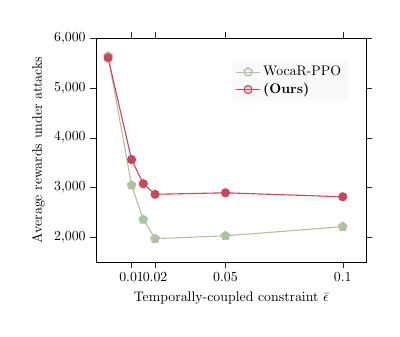
\begin{tikzpicture}[scale=0.5]

\definecolor{color0}{rgb}{0.917647058823529,0.917647058823529,0.949019607843137}
\definecolor{color1}{rgb}{0.372549019607843,0.619607843137255,0.627450980392157}
\definecolor{color2}{rgb}{0.133333333333333,0.545098039215686,0.133333333333333}
\definecolor{color3}{rgb}{0.576470588235294,0.43921568627451,0.858823529411765}
%\definecolor{color4}{rgb}{0.392156862745098,0.584313725490196,0.929411764705882}
%\definecolor{color5}{rgb}{0.862745098039216,0.0784313725490196,0.235294117647059}
\definecolor{color4}{HTML}{b1c2a3}
\definecolor{color5}{HTML}{C7495C}

\begin{axis}[
axis background/.style={fill=white},
axis line style={black},
legend cell align={left},
legend style={
  fill opacity=0.2,
  draw opacity=1,
  text opacity=1,
  at={(0.5,0.9)},
  anchor=north west,
  draw=none,
  fill=color0
},
tick align=outside,
x grid style={color=white},
xlabel={Temporally-coupled constraint $\bar{\epsilon}$},
xmajorgrids=false,
% xmajorticks=false,
xmin=-0.005, xmax=0.11,
xtick style={color=white!15!black},
xtick={ 0.01, 0.02, 0.05, 0.1},
xticklabels={ \num{0.01}, \num{0.02}, \num{0.05}, \num{0.1}},
y grid style={color=white},
ylabel={Average rewards under attacks},
ymajorgrids=false,
% ymajorticks=false,
ymin=1500, ymax=6000,
ytick style={color=white!15!black}
]
\addplot [line width=0.8pt, color4, color4, mark=pentagon*, mark size=3.2, mark options={solid}]
table{%
x  y
0  5638
0.01 3045
0.015 2356
0.02 1974
0.05 2030
0.1 2214
};
\addlegendentry{WocaR-PPO}
\addplot [line width=0.8pt, color5, mark=*, mark size=2.9, mark options={solid}]
table{%
x  y
0 5603
0.01 3561
0.015 3076
0.02 2864
0.05 2894
0.1 2814
};
\addlegendentry{\textbf{\ours(Ours)}}
\end{axis}
\end{tikzpicture}

    \vspace{-0.5em}
    \caption{Ablated studies for $\bar{\epsilon}$.
    % $\pi_\theta$ is the acting policy being trained by $\loss_{\pi_\theta}$ defined in Equation~\eqref{loss:policy}, including the original loss of the base DRL algorithm $\lossrl$, a regularization term $\lossreg$, as well as $\lossworst$, a term for improving the \worstqname based on $\worstcritic$. Here $\worstcritic$ which estimates the \worstqname of $\pi_\theta$ is updated by $\loss_{\worstcritic}=\lossest$ depending on $\pi_\theta$.  
    }
    \label{fig:eps_}
% \vspace{-1em}
\end{wrapfigure}
Conversely, setting $\bar{\epsilon}$ close to zero overly restricts perturbations, leading to a decline in attack performance. An appropriate value for $\bar{\epsilon}$ is critical for effective temporally-coupled attacks. Figure~\ref{fig:eps_} illustrates the performance of robust models against temporally-coupled state attackers trained with different maximum $\bar{\epsilon}$. For WocaR-PPO, the temporally-coupled attacker achieves optimal attack performance when the values of $\bar{\epsilon}$ are set to 0.02. As the $\bar{\epsilon}$ values increase and the temporally-coupled constraint weakens, the agent's performance improves, indicating a decrease in the adversary's attack effectiveness. In the case of \ours agents, they consistently maintain robust performance as the $\bar{\epsilon}$ values become larger. This observation highlights the impact of temporal coupling on the vulnerability of robust baselines to such attacks. In contrast, \ours agents consistently demonstrate robustness against these attacks.






